\subsection{Selezione Database}\label{SelectDB}

Al fine di collegare la rete bayesiana (caricata in §\ref{ReteB}) al flusso di monitoraggio l'utente deve selezionare il Database contente i dati da monitorare.\\
Tale operazione si articola in due passaggi fondamentali:
\begin{enumerate}
	\item \textbf{Passaggio 1:} L'utente seleziona, attraverso un menù a tendina, il database da usare come sorgente dati (Figura \ref{Sorgenti})
	\begin{figure}[H]
	\begin{center}
		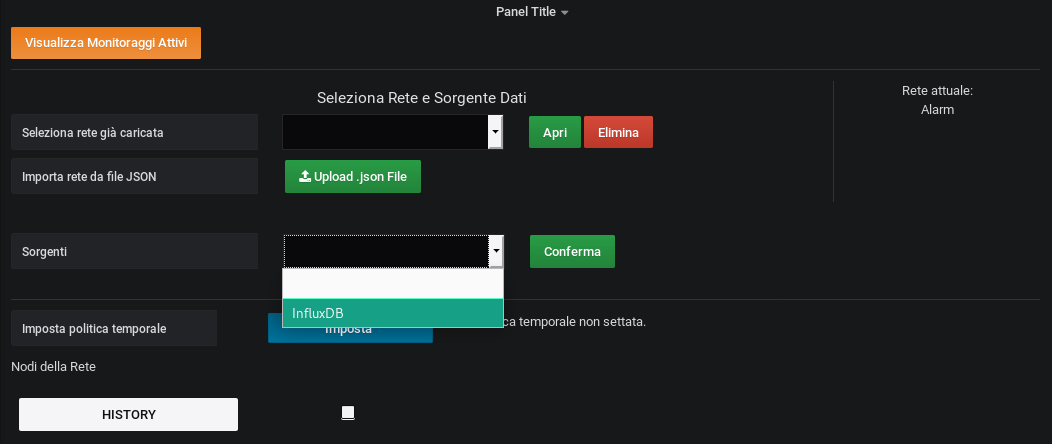
\includegraphics[scale=0.35]{./images/Sorgenti.png}
		 \caption{Elenco Database disponibili per il collegamento}	
		 \label{Sorgenti}
	\end{center}
	\end{figure}
	\item \textbf{Passagio 2:} L'utente conferma la propria scelta attraverso il pulsante \textbf{Conferma}, presente in Figura \ref{Sorgenti}
\end{enumerate}
~\\
Al seguito della corretta selezione del Database da usare come sorgente dati l'utente verrà avvisato del buon esito dell'operazione da un messaggio di notifica (Figura \ref{NotificaSorgente}). 

\begin{figure}[H]
	\begin{center}
		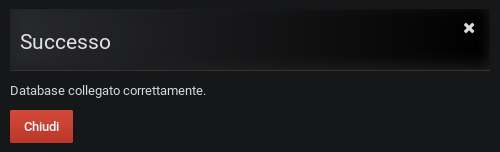
\includegraphics[scale=0.6]{./images/NotificaSorgente.png}
		 \caption{Notifica avvenuto collegamento Databse}	
		 \label{NotificaSorgente}
	\end{center}
\end{figure}